\documentclass{article}
\usepackage[margin=0.1in]{geometry}
\usepackage{pdflscape}
\usepackage{amssymb}
\usepackage{xcolor}
\usepackage{tikz}
\usetikzlibrary{positioning, shapes.geometric, calc}

% Define custom colors
\definecolor{darkblue}{RGB}{25,25,112}
\definecolor{lightblue}{RGB}{173,216,230}
\definecolor{darkred}{RGB}{139,0,0}
\definecolor{darkgreen}{RGB}{0,100,0}
\definecolor{purple}{RGB}{128,0,128}

\begin{document}
\thispagestyle{empty}
\begin{landscape}

\begin{center}
{\Huge\bfseries\color{darkblue} NINJAGO TRAINING}\\[0.3cm]
{\Large\itshape A Complex Choose Your Own Adventure Decision Tree}
\end{center}

\vspace{0.5cm}

\resizebox{1.15\textwidth}{!}{
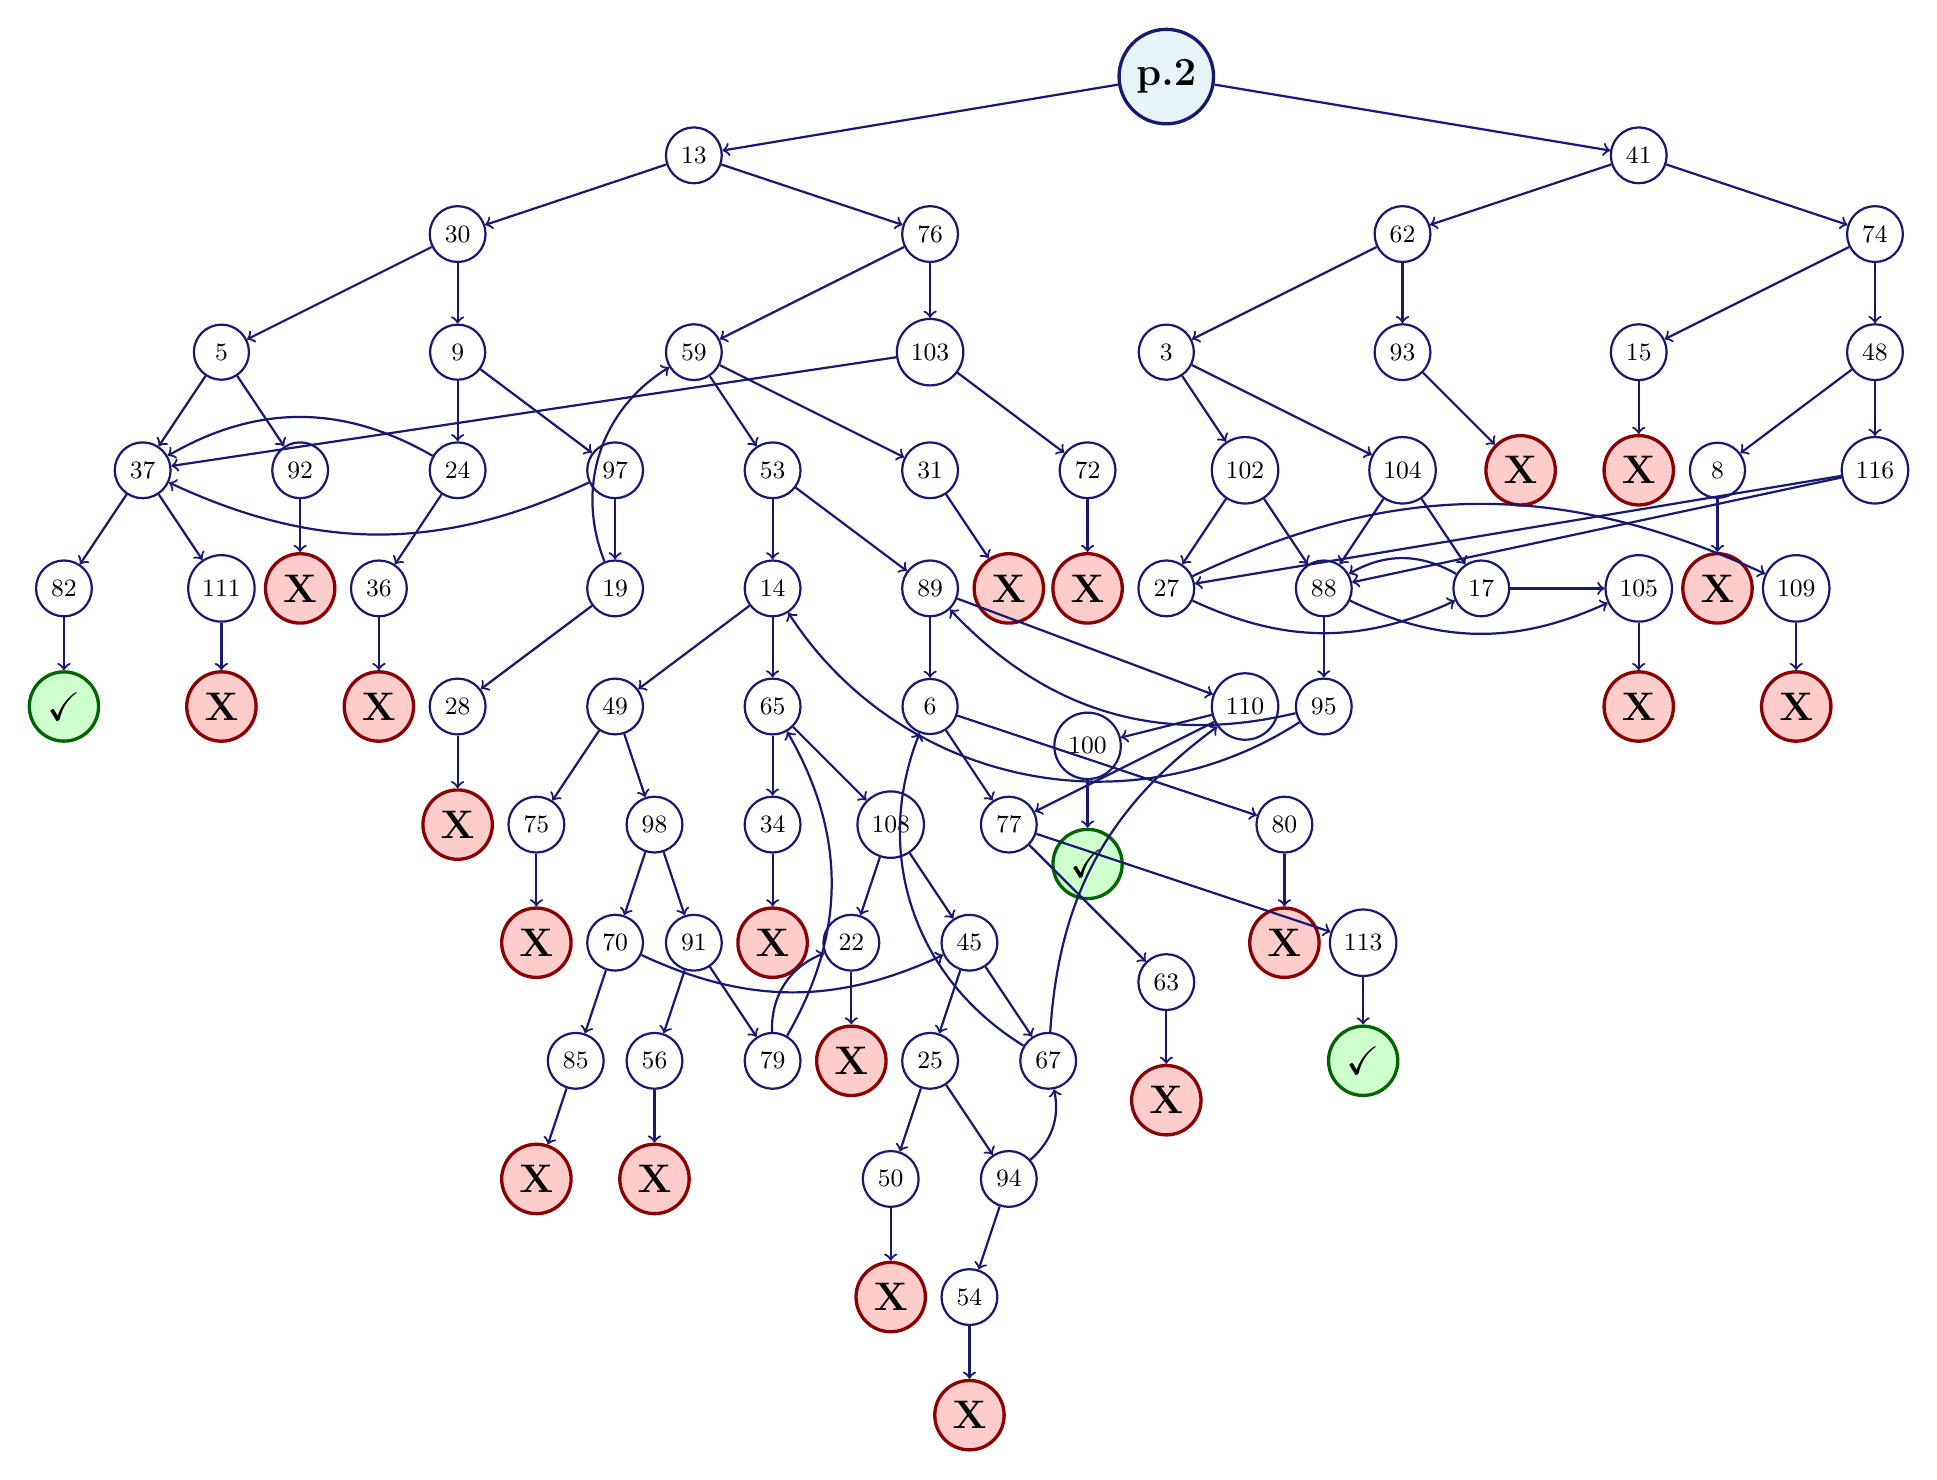
\begin{tikzpicture}[
    % Node styles
    start/.style={circle, draw=darkblue, fill=lightblue!30, minimum size=12mm, very thick, font=\Large\bfseries},
    page/.style={circle, draw=darkblue, minimum size=7mm, thick, font=\small},
    success/.style={circle, draw=darkgreen, fill=green!20, minimum size=7mm, very thick, font=\Large\bfseries},
    failure/.style={circle, draw=darkred, fill=red!20, minimum size=7mm, very thick, font=\Large\bfseries},
    % Edge styles
    edge/.style={draw=darkblue, thick, ->},
    backedge/.style={draw=darkblue, thick, ->}
]

% Level 0 - Start
\node[start] (p2) at (0,0) {p.2};

% Level 1
\node[page] (p13) at (-6,-1) {13};
\node[page] (p41) at (6,-1) {41};

% Level 2
\node[page] (p30) at (-9,-2) {30};
\node[page] (p76) at (-3,-2) {76};
\node[page] (p62) at (3,-2) {62};
\node[page] (p74) at (9,-2) {74};

% Level 3
\node[page] (p5) at (-12,-3.5) {5};
\node[page] (p9) at (-9,-3.5) {9};
\node[page] (p59) at (-6,-3.5) {59};
\node[page] (p103) at (-3,-3.5) {103};
\node[page] (p3) at (0,-3.5) {3};
\node[page] (p93) at (3,-3.5) {93};
\node[page] (p15) at (6,-3.5) {15};
\node[page] (p48) at (9,-3.5) {48};

% Level 4
\node[page] (p37) at (-13,-5) {37};
\node[page] (p92) at (-11,-5) {92};
\node[page] (p24) at (-9,-5) {24};
\node[page] (p97) at (-7,-5) {97};
\node[page] (p53) at (-5,-5) {53};
\node[page] (p31) at (-3,-5) {31};
\node[page] (p72) at (-1,-5) {72};
\node[page] (p102) at (1,-5) {102};
\node[page] (p104) at (3,-5) {104};
\node[page] (p8) at (7,-5) {8};
\node[page] (p116) at (9,-5) {116};

% Level 5
\node[page] (p82) at (-14,-6.5) {82};
\node[page] (p111) at (-12,-6.5) {111};
\node[page] (p36) at (-10,-6.5) {36};
\node[page] (p19) at (-7,-6.5) {19};
\node[page] (p14) at (-5,-6.5) {14};
\node[page] (p89) at (-3,-6.5) {89};
\node[page] (p27) at (0,-6.5) {27};
\node[page] (p88) at (2,-6.5) {88};
\node[page] (p17) at (4,-6.5) {17};
\node[page] (p105) at (6,-6.5) {105};
\node[page] (p109) at (8,-6.5) {109};

% Level 6
\node[page] (p28) at (-9,-8) {28};
\node[page] (p49) at (-7,-8) {49};
\node[page] (p65) at (-5,-8) {65};
\node[page] (p6) at (-3,-8) {6};
\node[page] (p110) at (1,-8) {110};
\node[page] (p95) at (2,-8) {95};
\node[page] (p100) at (-1,-8.5) {100};

% Level 7
\node[page] (p75) at (-8,-9.5) {75};
\node[page] (p98) at (-6.5,-9.5) {98};
\node[page] (p34) at (-5,-9.5) {34};
\node[page] (p108) at (-3.5,-9.5) {108};
\node[page] (p77) at (-2,-9.5) {77};
\node[page] (p80) at (1.5,-9.5) {80};

% Level 8
\node[page] (p70) at (-7,-11) {70};
\node[page] (p91) at (-6,-11) {91};
\node[page] (p22) at (-4,-11) {22};
\node[page] (p45) at (-2.5,-11) {45};
\node[page] (p63) at (0,-11.5) {63};
\node[page] (p113) at (2.5,-11) {113};

% Level 9
\node[page] (p85) at (-7.5,-12.5) {85};
\node[page] (p56) at (-6.5,-12.5) {56};
\node[page] (p79) at (-5,-12.5) {79};
\node[page] (p25) at (-3,-12.5) {25};
\node[page] (p67) at (-1.5,-12.5) {67};

% Level 10
\node[page] (p50) at (-3.5,-14) {50};
\node[page] (p94) at (-2,-14) {94};

% Level 11
\node[page] (p54) at (-2.5,-15.5) {54};

% Success nodes
\node[success] (win82) at (-14,-8) {$\checkmark$};
\node[success] (win100) at (-1,-10) {$\checkmark$};
\node[success] (win113) at (2.5,-12.5) {$\checkmark$};

% Failure nodes
\node[failure] (fail92) at (-11,-6.5) {X};
\node[failure] (fail111) at (-12,-8) {X};
\node[failure] (fail36) at (-10,-8) {X};
\node[failure] (fail28) at (-9,-9.5) {X};
\node[failure] (fail31) at (-2,-6.5) {X};
\node[failure] (fail72) at (-1,-6.5) {X};
\node[failure] (fail93) at (4.5,-5) {X};
\node[failure] (fail15) at (6,-5) {X};
\node[failure] (fail8) at (7,-6.5) {X};
\node[failure] (fail105) at (6,-8) {X};
\node[failure] (fail109) at (8,-8) {X};
\node[failure] (fail75) at (-8,-11) {X};
\node[failure] (fail34) at (-5,-11) {X};
\node[failure] (fail80) at (1.5,-11) {X};
\node[failure] (fail22) at (-4,-12.5) {X};
\node[failure] (fail63) at (0,-13) {X};
\node[failure] (fail85) at (-8,-14) {X};
\node[failure] (fail56) at (-6.5,-14) {X};
\node[failure] (fail50) at (-3.5,-15.5) {X};
\node[failure] (fail54) at (-2.5,-17) {X};

% Draw edges - Level 0-1
\draw[edge] (p2) -- (p13);
\draw[edge] (p2) -- (p41);

% Level 1-2
\draw[edge] (p13) -- (p30);
\draw[edge] (p13) -- (p76);
\draw[edge] (p41) -- (p62);
\draw[edge] (p41) -- (p74);

% Level 2-3
\draw[edge] (p30) -- (p5);
\draw[edge] (p30) -- (p9);
\draw[edge] (p76) -- (p59);
\draw[edge] (p76) -- (p103);
\draw[edge] (p62) -- (p3);
\draw[edge] (p62) -- (p93);
\draw[edge] (p74) -- (p15);
\draw[edge] (p74) -- (p48);

% Level 3-4
\draw[edge] (p5) -- (p37);
\draw[edge] (p5) -- (p92);
\draw[edge] (p9) -- (p24);
\draw[edge] (p9) -- (p97);
\draw[edge] (p59) -- (p53);
\draw[edge] (p59) -- (p31);
\draw[edge] (p103) -- (p37);
\draw[edge] (p103) -- (p72);
\draw[edge] (p3) -- (p102);
\draw[edge] (p3) -- (p104);
\draw[edge] (p93) -- (fail93);
\draw[edge] (p15) -- (fail15);
\draw[edge] (p48) -- (p8);
\draw[edge] (p48) -- (p116);

% Level 4-5
\draw[edge] (p37) -- (p82);
\draw[edge] (p37) -- (p111);
\draw[edge] (p92) -- (fail92);
\draw[edge] (p24) -- (p36);
\draw[backedge] (p24) to[bend right=30] (p37);
\draw[backedge] (p97) to[bend left=25] (p37);
\draw[edge] (p97) -- (p19);
\draw[edge] (p53) -- (p14);
\draw[edge] (p53) -- (p89);
\draw[edge] (p31) -- (fail31);
\draw[edge] (p72) -- (fail72);
\draw[edge] (p102) -- (p27);
\draw[edge] (p102) -- (p88);
\draw[edge] (p104) -- (p17);
\draw[edge] (p104) -- (p88);
\draw[edge] (p8) -- (fail8);
\draw[edge] (p116) -- (p27);
\draw[edge] (p116) -- (p88);

% Level 5-6
\draw[edge] (p82) -- (win82);
\draw[edge] (p111) -- (fail111);
\draw[edge] (p36) -- (fail36);
\draw[edge] (p19) -- (p28);
\draw[backedge] (p19) to[bend left=40] (p59);
\draw[edge] (p14) -- (p49);
\draw[edge] (p14) -- (p65);
\draw[edge] (p89) -- (p6);
\draw[edge] (p89) -- (p110);
\draw[backedge] (p27) to[bend right=25] (p17);
\draw[edge] (p27) to[bend left=25] (p109);
\draw[edge] (p88) -- (p95);
\draw[edge] (p88) to[bend right=25] (p105);
\draw[backedge] (p17) to[bend right=30] (p88);
\draw[edge] (p17) -- (p105);
\draw[edge] (p105) -- (fail105);
\draw[edge] (p109) -- (fail109);

% Level 6-7
\draw[edge] (p28) -- (fail28);
\draw[edge] (p49) -- (p75);
\draw[edge] (p49) -- (p98);
\draw[edge] (p65) -- (p34);
\draw[edge] (p65) -- (p108);
\draw[edge] (p6) -- (p77);
\draw[edge] (p6) -- (p80);
\draw[edge] (p110) -- (p77);
\draw[edge] (p110) -- (p100);
\draw[backedge] (p95) to[bend left=45] (p14);
\draw[backedge] (p95) to[bend left=30] (p89);
\draw[edge] (p100) -- (win100);

% Level 7-8
\draw[edge] (p75) -- (fail75);
\draw[edge] (p98) -- (p70);
\draw[edge] (p98) -- (p91);
\draw[edge] (p34) -- (fail34);
\draw[edge] (p108) -- (p22);
\draw[edge] (p108) -- (p45);
\draw[edge] (p77) -- (p63);
\draw[edge] (p77) -- (p113);
\draw[edge] (p80) -- (fail80);

% Level 8-9
\draw[backedge] (p70) to[bend right=25] (p45);
\draw[edge] (p70) -- (p85);
\draw[edge] (p91) -- (p56);
\draw[edge] (p91) -- (p79);
\draw[edge] (p22) -- (fail22);
\draw[edge] (p45) -- (p25);
\draw[edge] (p45) -- (p67);
\draw[edge] (p63) -- (fail63);
\draw[edge] (p113) -- (win113);

% Level 9-10
\draw[edge] (p85) -- (fail85);
\draw[edge] (p56) -- (fail56);
\draw[backedge] (p79) to[bend left=35] (p22);
\draw[backedge] (p79) to[bend right=30] (p65);
\draw[edge] (p25) -- (p50);
\draw[edge] (p25) -- (p94);
\draw[backedge] (p67) to[bend left=40] (p6);
\draw[backedge] (p67) to[bend left=25] (p110);

% Level 10-11
\draw[edge] (p50) -- (fail50);
\draw[edge] (p94) -- (p54);
\draw[backedge] (p94) to[bend right=30] (p67);

% Level 11-terminal
\draw[edge] (p54) -- (fail54);

\end{tikzpicture}
}

% \vspace{0.5cm}

% \begin{minipage}{0.45\textwidth}
% {\large\bfseries Legend:}\\[0.2cm]
% \begin{itemize}
% \item \textcolor{darkblue}{Blue circles}: Story pages
% \item \textcolor{lightblue}{Light blue circle}: Start
% \item \textcolor{darkgreen}{Green $\checkmark$}: Success ending
% \item \textcolor{darkred}{Red X}: Failure ending
% \item Solid arrows: All paths (including loops)
% \end{itemize}
% \end{minipage}
% \begin{minipage}{0.5\textwidth}
% {\large\bfseries Statistics:}
% \begin{itemize}
% \item Total pages: 64
% \item Maximum depth: 12 levels
% \item Success paths: 3
% \item Failure paths: 21
% \item Loop edges: 13
% \end{itemize}
% \end{minipage}

\end{landscape}
\end{document}